\label{sec:noise_simulation}

查看本节演示代码：\demonotebook{03}{chapt03} \ \demonotebookgithub{03}{chapt03}

\subsubsection{量子信道}
由于量子退相干以及与环境的耦合，当前量子计算机在计算过程中经常发生误差。这些误差会出现在态制备、量子门操作和测量等阶段，通常称为量子噪声。量子噪声可以由量子信道刻画。在量子信息理论中，量子信道是指算符空间中的完全正定保迹（CPTP）映射，也可视为一种量子操作。所有量子信道都可以由 Kraus 算符表示：

\begin{equation}
    \Psi(\rho) = \sum_i K_i \rho K_i^\dagger,
\end{equation}

其中，$\Psi$ 为量子信道，$\rho$ 为密度矩阵，$\{K_i\}$ 为 $\Psi$ 的 Kraus 算符。Kraus 算符满足完备性条件：

\begin{equation}
    \sum_i K_i^\dagger K_i = I.
\end{equation}

在密度矩阵模拟器 \code{"mqmatrix"} 中，我们支持基于上述数学形式模拟量子信道。除密度矩阵方法外，在 \MindQuantum\ 的状态矢量模拟器 \code{"mqvector"} 中，我们也支持使用 Monte Carlo 方法模拟量子信道。噪声门会以一定概率影响量子比特。通过对线路进行多次采样，可以得到包含噪声的量子线路模拟结果。这个过程更加接近真实量子计算机的工作方式。

\MindQuantum\ 中实现了以下量子信道。

\PauliChannel：Pauli 信道可以看作 Pauli 算符按照某一概率分布随机作用于量子态 $\rho$。
\begin{equation}
    \Psi(\rho) = (1-p_x-p_y-p_z) \rho + p_x X \rho X + p_y Y \rho Y + p_z Z \rho Z.
\end{equation}
如果只有 $p_x$ 非零，它就成为 \BitFlipChannel。类似地，\PhaseFlipChannel\ 只有 $p_z$ 一个非零值，而 \BitPhaseFlipChannel\ 中非零的是 $p_y$。一个特殊情形是所有 Pauli 算符具有相同概率，这称为 \DepolarizingChannel。退极化信道广泛用于描述量子噪声。以下是一量子比特情形下的公式：
\begin{equation}
    \Psi(\rho) =  (1-p) \rho + \frac{p}{4}(I\rho I+X\rho X+Y\rho Y+Z\rho Z).
\end{equation}
\MindQuantum\ 中的退极化信道也支持多量子比特情形。
\begin{lstlisting}
from mindquantum.core.gates import DepolarizingChannel
from mindquantum.core.circuit import Circuit
circ = Circuit()
circ += DepolarizingChannel(0.02).on(0)
circ += DepolarizingChannel(0.01, 2).on([0, 1])
\end{lstlisting}

阻尼信道：常见的阻尼信道包括 \AmplitudeDampingChannel\ 和 \PhaseDampingChannel。振幅阻尼信道可以描述系统能量耗散，而相位阻尼信道描述的是不与环境交换能量时量子信息的损失。
振幅阻尼信道施加噪声的形式为：
\begin{gather*}
    \epsilon(\rho) = E_0 \rho E_0^\dagger + E_1 \rho E_1^\dagger
    \\
    \text{其中}\ {E_0}=\begin{bmatrix}1 & 0               \\
        0 & \sqrt{1-\gamma}\end{bmatrix},
    \ {E_1}=\begin{bmatrix}0 & \sqrt{\gamma} \\
        0 & 0\end{bmatrix}.
\end{gather*}
相位阻尼信道施加噪声的形式为：
\begin{gather*}
    \epsilon(\rho) = E_0 \rho E_0^\dagger + E_1 \rho E_1^\dagger
    \\
    \text{其中}\ {E_0}=\begin{bmatrix}1 & 0               \\
        0 & \sqrt{1-\gamma}\end{bmatrix},
    \ {E_1}=\begin{bmatrix}0 & 0             \\
        0 & \sqrt{\gamma}\end{bmatrix}.
\end{gather*}

\KrausChannel：这是 \MindQuantum\ 中的自定义单量子比特量子信道，可以通过传入 Kraus 算符构造。
\begin{lstlisting}
from mindquantum.core.gates import KrausChannel
from mindquantum.core.circuit import Circuit
from cmath import sqrt
gamma = 0.5
kmat0 = [[1, 0], [0, sqrt(1 - gamma)]]
kmat1 = [[0, sqrt(gamma)], [0, 0]]
amplitude_damping = KrausChannel('damping', [kmat0, kmat1])
circ = Circuit()
circ += amplitude_damping.on(0)
\end{lstlisting}

\subsubsection{Channel Adder}
真实量子芯片由多个量子比特组成。由于制造过程中的固有差异，每个量子比特都会表现出不同误差来源。此外，即使是同一个量子比特，在施加不同量子门时对应误差也会发生变化。为了忠实复现量子芯片中的固有误差，需要精心设计精确的误差模型。在 \MindQuantum\ 中，我们开发了一组名为 Channel Adder（信道添加器）的工具，用于快速构建噪声模型。通过 Channel Adder，可以方便地在不同量子门之后引入不同量子信道，并针对特定量子比特进行定制，再利用含噪模拟器模拟这些噪声模型。

\ChannelAdder\ 类主要由三个函数组成：\code{_accepter()}、\code{_excluder()} 和 \code{_handler(BasicGate)}。它们的功能如下：
\begin{itemize}
    \item \code{_accepter()}：返回一个函数列表，称为接受规则集；其中每个接受规则函数都以量子门作为输入。当函数返回 True 时，表示可以在该量子门之后添加信道。
    \item \code{_excluder()}：返回一个函数列表，称为拒绝规则集；其中每个拒绝规则函数都以量子门作为输入。当函数返回 True 时，表示拒绝在该量子门之后添加信道。
    \item \code{_handler(BasicGate)}：以量子门作为输入，并返回一个量子线路，用于表示添加在输入量子门之后的自定义信道。
\end{itemize}

以 \BitFlipAdder\ 为例。该添加器会在每个量子门之后添加一个比特翻转信道。
\begin{lstlisting}
from mindquantum.core.circuit import Circuit, BitFlipAdder

circ = Circuit().h(0).rx('a', 1).z(1, 0)
noise_model = BitFlipAdder(0.3, with_ctrl=False)
noise_circ = noise_model(circ)
print(noise_model)
\end{lstlisting}
输出为：
\begin{lstlisting}
BitFlipAdder<flip_rate=0.3, with_ctrl=False>
\end{lstlisting}
将该噪声模型应用到线路后，每个量子门之后都会添加一个比特翻转信道，如图~\ref{fig:bit_flip_adder} 所示。
\begin{figure}
    \centering
    \begin{subfigure}{0.2\textwidth}
        \centering
        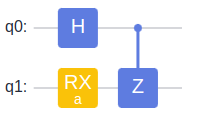
\includegraphics[width=\textwidth]{images/3_3_no_bit_fip.png}
        \caption{无噪声线路。}
    \end{subfigure}
    \begin{subfigure}{0.4\textwidth}
        \centering
        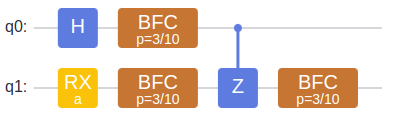
\includegraphics[width=0.9\textwidth]{images/3_3_bit_fip.png}
        \caption{经过 \texttt{BitFlipAdder} 处理后的线路。}
    \end{subfigure}
    \caption{将 BitFlipAdder 应用于量子线路的示例。}
    \label{fig:bit_flip_adder}
\end{figure}

下面给出一个更复杂的示例，以展示 Channel Adder 的能力。假设量子芯片上不同量子比特的单量子比特门操作噪声可以忽略不计，并考虑两量子比特门在不同量子比特上表现出不同的退极化信道。此外，线路测量会受到比特翻转误差影响，翻转概率为 0.01。假设不同量子比特上的退极化信道为：
\begin{lstlisting}
from mindquantum.core import *
dc0 = DepolarizingChannel(0.01)
dc1 = DepolarizingChannel(0.02)
dc2 = DepolarizingChannel(0.03)
\end{lstlisting}
接下来按如下方式构建完整噪声模型：
\begin{lstlisting}
adder1 = MixerAdder([
    NoiseExcluder(),
    ReverseAdder(MeasureAccepter()),
    QubitNumberConstrain(2),
    NoiseChannelAdder(dc0, focus_on=0),
])
adder2 = MixerAdder([
    NoiseExcluder(),
    ReverseAdder(MeasureAccepter()),
    QubitNumberConstrain(2),
    NoiseChannelAdder(dc1, focus_on=1),
])
adder3 = MixerAdder([
    NoiseExcluder(),
    ReverseAdder(MeasureAccepter()),
    QubitNumberConstrain(2),
    NoiseChannelAdder(dc2, focus_on=2),
])
adder4 = MixerAdder([
    NoiseExcluder(),
    MeasureAccepter(),
    BitFlipAdder(0.01)
], add_after=False)

noise_model = SequentialAdder([
    adder1,
    adder2,
    adder3,
    adder4
])
print(noise_model)
\end{lstlisting}
输出为：
\begin{lstlisting}
SequentialAdder<
  MixerAdder<
    NoiseExcluder<>
    ReverseAdder<
      MeasureAccepter<>
    >
    QubitNumberConstrain<n_qubits=2, with_ctrl=True>
    NoiseChannelAdder<channel=DC(p=1/100), with_ctrl=True>
  >
  MixerAdder<
    NoiseExcluder<>
    ReverseAdder<
      MeasureAccepter<>
    >
    QubitNumberConstrain<n_qubits=2, with_ctrl=True>
    NoiseChannelAdder<channel=DC(p=1/50), with_ctrl=True>
  >
  MixerAdder<
    NoiseExcluder<>
    ReverseAdder<
      MeasureAccepter<>
    >
    QubitNumberConstrain<n_qubits=2, with_ctrl=True>
    NoiseChannelAdder<channel=DC(p=0.03), with_ctrl=True>
  >
  MixerAdder<
    NoiseExcluder<>
    MeasureAccepter<>
    BitFlipAdder<flip_rate=0.01, with_ctrl=True>
  >
>
\end{lstlisting}
\MixerAdder\ 是一组添加器，只有满足所有 \code{_accepter()} 和 \code{_excluder()} 规则时才会生效。\SequentialAdder\ 中的所有 Channel Adder 会逐一执行。从图~\ref{fig:complex_adder} 可以看出，该噪声模型满足我们的需求。

% \begin{lstlisting}
% circ = Circuit().rx('a', 0).rx('b', 1).x(1, 0).rz('c', 1).x(1, 0).measure_all()
% \end{lstlisting}
\begin{figure}
    \centering
    \begin{subfigure}{0.32\textwidth}
        \centering
        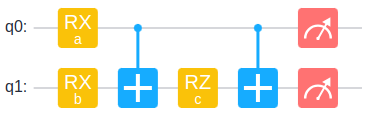
\includegraphics[width=\textwidth]{images/3_3_no_complex.png}
        \caption{无噪声线路。}
    \end{subfigure}
    \begin{subfigure}{0.5\textwidth}
        \centering
        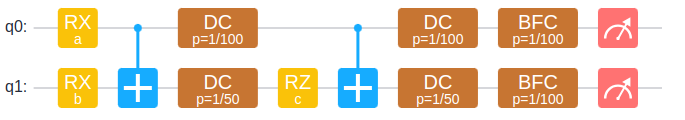
\includegraphics[width=\textwidth]{images/3_3_complex.png}
        \caption{经过复合 Channel Adder 处理后的线路。}
    \end{subfigure}
    \caption{将复合 Channel Adder 应用于量子线路的示例。}
    \label{fig:complex_adder}
\end{figure}

构建噪声模型后，可以在 \MindQuantum\ 中很方便地使用该噪声模型模拟量子线路。
\begin{lstlisting}
circ = Circuit().rx('a', 0).rx('b', 1).x(1, 0).rz('c', 1).x(1, 0).measure_all()
noise_sim = Simulator(NoiseBackend('mqvector', 2, noise_model))
noise_sim.sampling(circ, pr={'a': 1, 'b': 2, 'c':3}, shots=10000)
\end{lstlisting}
这里，我们使用基于 \code{"mqvector"} 的 \NoiseBackend\ 和此前构建的噪声模型，构造了一个噪声模拟器。
